% TODO:

% Write ``Liquid-vapor interface'' section A.

% Look up question-mark references (citations).

\documentclass[letterpaper,twocolumn,amsmath,amssymb,prb]{revtex4-1}
\usepackage{graphicx}% Include figure files
\usepackage{dcolumn}% Align table columns on decimal point
\usepackage{bm}% bold math
\usepackage{color}

\newcommand{\red}[1]{{\bf \color{red} #1}}
\newcommand{\blue}[1]{{\bf \color{blue} #1}}
\newcommand{\green}[1]{{\bf \color{green} #1}}
\newcommand{\rr}{\textbf{r}}
\newcommand{\xx}{\textbf{x}}
\newcommand{\refnote}{\red{[ref]}}

\newcommand{\fixme}[1]{\red{[#1]}}

% needsworklater is used to annotate bits that need work, but that we
% can postpone for a while.
\newcommand{\needsworklater}[1]{\emph{[#1]}}
% needsworknow is intended to prioritize stuff that needs fixing.
\newcommand{\needsworknow}[1]{\textcolor{red}{[\emph{#1}]}}

\begin{document}
\title{A Fundamental Measure Theory Functional for Hard-Sphere Contact Densities}

\author{David Roundy}
\affiliation{Department of Physics, Oregon State University, Corvallis, OR 97331}

%%%%%%%%%%%%%%%%%%%%%%%%%%%%%%%%%%%%%%%%%%%%%%%%%%%%%%%%%%%%
\begin{abstract}
\needsworklater{ We develop a functional based on FMT to ... for SAFT}
\end{abstract}

\maketitle

%%%%%%%%%%%%%%%%%%%%%%%%%%%%%%%%%%%%%%%%%%%%%%%%%%%%%%%%%%%%
\section{Introduction}

\cite{roth2002whitebear}

The hard-sphere contact density---which we will define as the density
of hard spheres touching a given hard sphere---is important for the
association term in Statistical Associating Fluid Theory (SAFT).  For
a homogeneous hard-sphere fluid, the contact density---which is to
say, $n g_{HS}(\sigma)$---is easily computed from the
Carnahan-Starling equation of state
\begin{align}
  g_{HS}(\sigma) &= \frac{1}{1-\eta} + \cdots
\end{align}
The contact density may be easily computed from a knowledge of the
contact theorem, which states that the pressure on any hard surface is
given by
\begin{align}
  p &= k_BT n_\textit{contact}
\end{align}
Since we are interested in the contact density at the hard-sphere
surface, all we need compute is the pressure on that surface, and
we'll have our answer.  The pressure on a hard sphere can be readily
computed from the dependence of the free energy on hard sphere
radius.
\begin{align}
  A_{HS} &= Nk_BT \frac{4\eta - 3\eta^2}{(1-\eta)^2}
\end{align}
Since $\eta \equiv \frac{4\pi}{3} R^3$, we can work out that
\begin{align}
  \frac{dA_{HS}}{dR} &= \frac{dA_{HS}}{d\eta} \frac{d\eta}{dR} \\
  &= Nk_BT \left( \frac{4 - 6\eta}{(1-\eta)^2} + 2 \frac{4\eta - 3\eta^2}{(1-\eta)^3} \right) \frac{d\eta}{dR}
  \\
  &= Nk_BT \frac{4 - 4\eta - 6\eta + 6\eta^2 + 8\eta - 6\eta^2}{(1-\eta)^3} \frac{d\eta}{dR}
  \\
  &= Nk_BT \frac{4 - 2\eta}{(1-\eta)^3} \frac{d\eta}{dR}
  \\
  &= Nk_BT \frac{4 - 2\eta}{(1-\eta)^3} \frac{3 \eta}{R}
\end{align}
This derivative gives us the force on \emph{all} the hard
spheres---since we're changing all their radii at once.  To compute
the pressure on the spheres, we just need to divide by the total area,
which means dividing by $N 4\pi (2R)^2$.  The area which is relevant
is the area over which the molecules can make contact.
\begin{align}
  p_{HS} &= \frac{1}{N 4\pi (2R)^2} \frac{dA_{HS}}{dR} \\
  &= \frac14 \frac{1}{N 4\pi R^2} Nk_BT \frac{4 - 2\eta}{(1-\eta)^3} \frac{3 \eta}{R} \\
  &= \frac{3}{4\pi R^3} \eta k_BT \frac{1 - \frac{\eta}2}{(1-\eta)^3} \\
  &= n k_BT \frac{1 - \frac{\eta}2}{(1-\eta)^3} \\
  n_\textit{contact} &= n \frac{1 - \frac{\eta}2}{(1-\eta)^3} \\
  g_{HS}(\sigma) &= \frac{1 - \frac{\eta}2}{(1-\eta)^3}
\end{align}
As it turns out, this is the correct answer! $\ddot\smile$

\section{Contact density at a given hard sphere}

When we consider an inhomogeneous system, we may ask for \emph{which}
sphere we are interested in computing the contact density.  One way to
answer this is to specify a sphere at a fixed position $\mathbf{r}$.
By making the hard-sphere radius dependent on position, we can compute
the pressure on the hard spheres located at $\mathbf{r}$.
\begin{align}
  p_{HS}(\mathbf{r}) &= \frac{1}{4\pi (2R)^2} \frac{\delta A_{HS}}{\delta R(\mathbf{r})}
\end{align}
So to compute this we need
\begin{align}
  \frac{\delta A_{HS}}{\delta R(\mathbf{r})} &=
  \int \left(
  \frac{\delta A_{HS}}{\delta n_3(\mathbf{r}')}
  \frac{\delta n_3(\mathbf{r}')}{\delta R(\mathbf{r})}
  +
  \frac{\delta A_{HS}}{\delta n_2(\mathbf{r}')}
  \frac{\delta n_2(\mathbf{r}')}{\delta R(\mathbf{r})}
  + \cdots
  \right) d\mathbf{r}'
\end{align}
There are \emph{many} such terms, but none of them are particularly
challenging.

\begin{figure}
\includegraphics[width=3cm]{figs/n0}
\caption{Set of hard spheres that included in $n_0(\mathbf{r})$.}
\label{fig:n0}
\end{figure}

\section{Contact density at a given contact position}

Unfortunately, knowing the average contact density on each hard sphere
doesn't really give us what we want for SAFT.  The trouble is that in
order to work out the fraction of association sites occupied, we need
to know the contact density \emph{at the point of contact}.
Fortunately, we don't need to know the contact density for a
particular sphere at each point of contact.  Just as $n_0(\mathbf{r})$
gives us the density of spheres that are contacting point $\mathbf{r}$
(see Figure~\ref{fig:n0}, we can use similar reasoning to work out the
contact density for these spheres.

To find the contact density at a given point of contact, we can't
simply change the radius for spheres touching that point, since that
would give us the pressure averaged over the entire surface of those
spheres.  Instead, we'll have to imagine extending a patch of those
spheres which is located at the point of interest.

\begin{figure}
\includegraphics[width=3cm]{figs/contact}
\caption{Construction for finding the contact density at a given point
  of contact.}
\label{fig:contact}
\end{figure}

%%%%%%%%%%%%%%%%%%%%%%%%%%%%%%%%%%%%%%%%%%%%%%%%%%%%%%%%%%%%
\section{Conclusion}
We get a nice spatial dependence for SAFT.

\bibliography{paper}% Produces the bibliography via BibTeX.

\end{document}

